\documentclass{article}

%\usepackage[math,lf,footnotefigures]{MyriadPro}
%\renewcommand{\familydefault}{\sfdefault}
\newcommand*{\mytextstyle}{\sffamily\Large\bfseries\color{black!85}}
%\usepackage[T1]{fontenc}

\usepackage{tikz}
\usetikzlibrary{arrows}
\usetikzlibrary{arrows.meta}
\usetikzlibrary{positioning}
\usetikzlibrary{decorations.text}

\usepackage{xcolor}
\definecolor{ufzgray1}{RGB}{126,126,126}
\definecolor{ufzgray2}{RGB}{156,156,156}
\definecolor{ufzgray3}{RGB}{185,185,185}
\definecolor{ufzgray4}{RGB}{230,230,230}

\usepackage{enumitem}

% adjust the page margins
\usepackage[left=2.7cm,right=2.5cm,top=1.2cm,bottom=1cm]{geometry}

\begin{document}
	
	\pagestyle{empty}
	
	\hspace*{-3cm}
	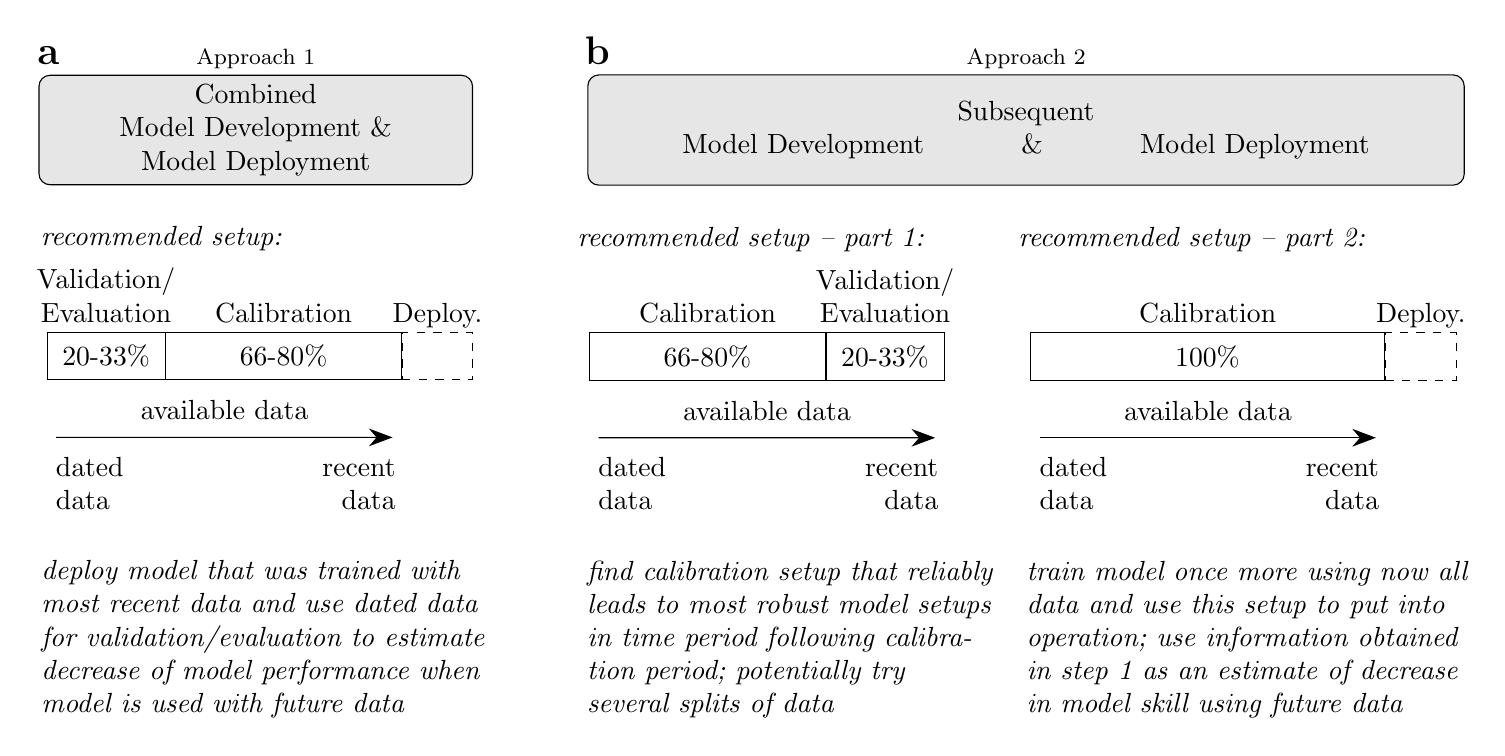
\begin{tikzpicture}[scale=2.5]
	
		\tikzstyle{block} = [rectangle, draw, fill=white!20, text centered, rounded corners, minimum height=1em]
		\tikzstyle{blockwide} = [rectangle, draw, fill=white!20, 
		text width=14.5em, text centered, rounded corners, minimum height=1em]
		\tikzstyle{noblock} = [rectangle, %fill=white!20, 
		text width=27.0em, rounded corners, minimum height=1em]
		\tikzstyle{noblockwide} = [rectangle, %fill=white!20, 
		text width=14.5em, rounded corners, minimum height=1em]
		\tikzstyle{abcblock} = [rectangle, fill=white!20, 
		text width=1em, rounded corners, minimum height=1em]
		\tikzstyle{line} = [draw, -latex']
		\tikzstyle{line} = [draw,latex'-latex'new]
	
		% combined
		\node [block,text width=15em,align=center,xshift=0.0cm,fill=ufzgray4] (a1) {Combined\\Model Development \&\\Model Deployment};
		\node [above=-0.05cm of a1.north,align=center] {\footnotesize Approach 1};
		\node [above=0.0cm of a1.north,align=left,xshift=-7.5em,font=\bfseries] {\Large{a}};
		
		\node [below=0.4cm of a1.south,align=center,xshift=-1.2cm,font=\itshape] (a2) {recommended setup:};
		
		% rectangles
		\node [below=0.9cm of a2.south,draw,rectangle,minimum width=1.5cm,minimum height=0.6cm,label={[align=center]Validation/\\Evaluation},xshift=-0.7cm] (a3a) {20-33\%};
		\node [right=0.4cm of a3a.east,draw,rectangle,minimum width=3.0cm,minimum height=0.6cm,label=Calibration,xshift=-0.41cm] (a3b) {66-80\%};
		\node [right=0.4cm of a3b.east,draw,rectangle,minimum width=0.9cm,minimum height=0.6cm,label={[label distance=-0.07cm]Deploy.},xshift=-0.41cm,dashed] (a3c) {};
		\node [right=0.4cm of a3a.east,draw,rectangle,minimum width=3.0cm,minimum height=0.6cm,label=,xshift=-0.41cm] (a3b) {};
		
		% Arrow
		\node [below=0.6cm of a3a.south west] (startarrow) {};
		\node [below=0.6cm of a3b.south east] (endarrow) {};
		\node [below=0.0cm of startarrow.south,align=left,xshift=0.55cm] (a4a) {dated\\data};
		\node [below=0.03cm of endarrow.south,align=right,xshift=-0.55cm] (a4b) {recent\\data};
		\draw [-{Stealth[length=3mm]}] (startarrow) -- node[above=1mm] {available data} (endarrow) ;
		
		\node [below=0.4cm of a4a.south,align=left,xshift=2.2cm,font=\itshape] (a5) {deploy model that was trained with \\most recent data and use dated data\\ for validation/evaluation to estimate\\ decrease of model performance when\\model is used with future data };
		
		% Subsequent
		\node [block,text width=31em,align=center,minimum height=1.4cm,xshift=0.0cm,right=1.45cm of a1.east,fill=ufzgray4] (b1) {Subsequent\\Model Development \hspace*{1.0cm} \& \hspace*{1.0cm} Model Deployment};
		\node [above=-0.05cm of b1.north,align=center] {\footnotesize Approach 2};
		\node [above=0.0cm of b1.north,align=left,xshift=-15.5em,font=\bfseries] {\Large{b}};
		
		\node [below=0.4cm of b1.south,align=center,xshift=-3.5cm,font=\itshape] (b2) {recommended setup -- part 1:};
		
		% rectangles
		\node [below=0.9cm of b2.south,draw,rectangle,minimum width=3.0cm,minimum height=0.6cm,label=Calibration,xshift=-0.55cm] (b3a) {66-80\%};
		\node [right=0.4cm of b3a.east,draw,rectangle,minimum width=1.5cm,minimum height=0.6cm,label={[align=center]Validation/\\Evaluation},xshift=-0.41cm] (b3b) {20-33\%};
		
		% Arrow
		\node [below=0.6cm of b3a.south west] (startarrow2) {};
		\node [below=0.6cm of b3b.south east] (endarrow2) {};
		\node [below=0.0cm of startarrow2.south,align=left,xshift=0.55cm] (b4a) {dated\\data};
		\node [below=0.03cm of endarrow2.south,align=right,xshift=-0.55cm] (b4b) {recent\\data};
		\draw [-{Stealth[length=3mm]}] (startarrow2) -- node[above=1mm] {available data} (endarrow2) ;
		
		\node [below=0.4cm of b4a.south,align=left,xshift=2.0cm,font=\itshape] (b5) {find calibration setup that reliably\\  leads to most robust model setups\\ in time period following calibra-\\ tion period; potentially try \\ several splits of data};
		
		
		\node [below=0.4cm of b1.south,align=center,xshift=2.1cm,font=\itshape] (bb2) {recommended setup -- part 2:};
		
		% rectangles
		\node [below=0.9cm of bb2.south,draw,rectangle,minimum width=4.5cm,minimum height=0.6cm,label=Calibration,xshift=0.2cm] (bb3a) {100\%};
		\node [right=0.4cm of bb3a.east,draw,rectangle,minimum width=0.9cm,minimum height=0.6cm,label={[label distance=-0.07cm]Deploy.},xshift=-0.41cm,dashed] (bb3c) {};
		\node [below=0.9cm of bb2.south,draw,rectangle,minimum width=4.5cm,minimum height=0.6cm,label=,xshift=0.2cm] (bb3a) {};
		
		% Arrow
		\node [below=0.6cm of bb3a.south west] (startarrow3) {};
		\node [below=0.6cm of bb3a.south east] (endarrow3) {};
		\node [below=0.0cm of startarrow3.south,align=left,xshift=0.55cm] (bb4a) {dated\\data};
		\node [below=0.03cm of endarrow3.south,align=right,xshift=-0.55cm] (bb4b) {recent\\data};
		\draw [-{Stealth[length=3mm]}] (startarrow3) -- node[above=1mm] {available data} (endarrow3) ;
		
		\node [below=0.4cm of bb4a.south,align=left,xshift=2.2cm,font=\itshape] (bb5) {train model once more using now all \\data and use this setup to put into \\ operation; use information obtained\\ in step 1 as an estimate of decrease  \\ in model skill using future data};
				
	\end{tikzpicture}
	
\end{document}



